\documentclass[11pt]{article}
\usepackage[margin=1.6cm]{geometry}
\usepackage{graphicx}
\usepackage{booktabs}
\usepackage{xcolor}
\usepackage{colortbl}
\usepackage{array}
\usepackage{tabularx}
\usepackage{hyperref}
\hypersetup{colorlinks=true,linkcolor=blue!50!black,citecolor=blue!50!black}

\definecolor{good}{RGB}{0,120,0}
\definecolor{bad}{RGB}{200,40,40}
\definecolor{withheldbg}{RGB}{255,245,200}

\newcommand{\good}[1]{\textcolor{good}{\textbf{#1}}}
\newcommand{\bad}[1]{\textcolor{bad}{\textbf{#1}}}
\newcommand{\wh}[1]{\cellcolor{withheldbg}#1}

\setlength{\parindent}{0pt}
\setlength{\parskip}{4pt}

\title{\textbf{EOLLM Task Ablation Study}\\[2pt]
\large Qwen3.5-4B-VL on EOLLM urban VQA --- Apr 26--30, 2026}
\author{Ezel Bayraktar}
\date{}

\begin{document}
\maketitle
\vspace{-1.2cm}

\section*{TL;DR}
\begin{itemize}\itemsep1pt
\item Removing tasks does not improve kept tasks. Every ablation underperforms PC-base on its own kept subset.
\item Withheld-task transfer is partial and asymmetric. mismatch\_mcq + camera\_direction collapse to chance when their family is fully withheld.
\item Withholding only the \emph{hard} half of a family (Split-6) preserves $>$80\% on the hard variant: easy/hard mismatch share representation.
\item Withholding camera\_direction alone (Split-5) leaves it at chance (29.9\%, random=25); zero transfer from urban/mismatch supervision.
\item Cross-city baseline (SU-base) is genuinely harder: 70.8\% vs PC-base 78.3\%.
\item green\_space and road\_surface stay at $\sim$94--100\% in every PC run --- leakage, not learning.
\item Split-2a regressed: ep1 59.5\% $\to$ ep3 50.7\%. Removing both mismatch and camera\_dir destabilizes training.
\item More epochs do not close the withheld-task gap (Split-1 plateaus by ep4).
\end{itemize}

\section{Run matrix}

\begin{table}[h]\centering\small
\setlength{\tabcolsep}{4pt}
\begin{tabular}{l l p{8cm} c c}
\toprule
\textbf{Run} & \textbf{Split} & \textbf{Topics removed from training} & \textbf{Epochs} & \textbf{Status} \\
\midrule
PC-base   & per\_city    & none                                                                         & 6 & \good{done} \\
SU-base   & seen\_unseen & none                                                                         & 8 & \good{done} \\
Split-1   & per\_city    & 7 urban: amenity, bldg\_h, junction, land\_use, road\_type, transit, urban\_density & 5 & \good{done} \\
Split-2a  & per\_city    & 5 geo: camera\_direction, all 4 mismatch\_*                                  & 3 & \good{done} (regressed) \\
Split-2b  & seen\_unseen & 5 geo: camera\_direction, all 4 mismatch\_*                                  & 5 & \good{done} \\
Split-3   & per\_city    & 4 mismatch\_* only (camera\_dir kept)                                        & 5 & \good{done} \\
Split-5   & per\_city    & camera\_direction only                                                       & 5 & \good{done} \\
Split-6   & per\_city    & mismatch\_binary\_hard + mismatch\_mcq\_hard (easy variants kept)            & 5 & \good{done} \\
\bottomrule
\end{tabular}
\end{table}

Eval = all 14 topics in every run. bs=96, LoRA r=16/$\alpha$=16, lr=2.5e-4, RTX Pro 6000 96 GB.

\section{Headline}

\begin{figure}[h]\centering
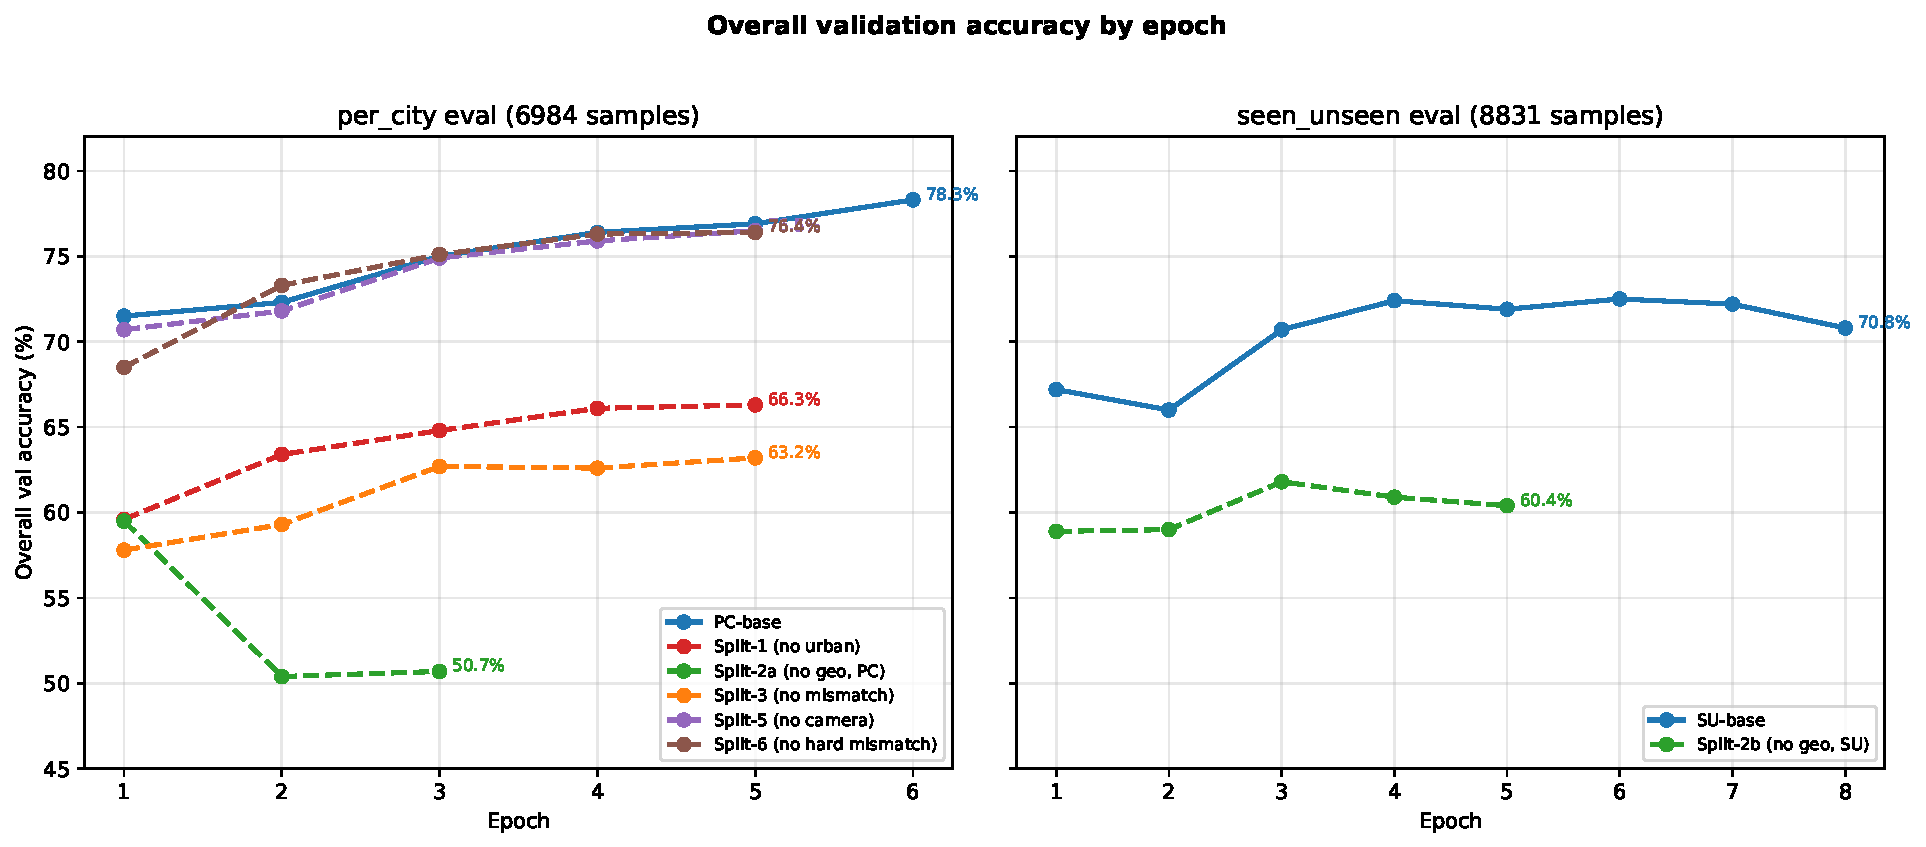
\includegraphics[width=\textwidth]{figures/fig1_overall.pdf}
\end{figure}

\begin{itemize}\itemsep1pt
\item PC-base ends at 78.3\%, still rising.
\item Every per\_city ablation underperforms the full baseline on the same eval.
\item SU-base (70.8\%) is the honest cross-city number, $\sim$7.5 pp below PC-base.
\end{itemize}

\newpage
\section{Per-topic final accuracy}

\begin{table}[h]\centering\footnotesize
\setlength{\tabcolsep}{3.5pt}
\renewcommand{\arraystretch}{1.05}
\begin{tabular}{l c c c c c c c c}
\toprule
\textbf{Topic} & \textbf{PC-base} & \textbf{SU-base} & \textbf{Split-1} & \textbf{Split-2a} & \textbf{Split-2b} & \textbf{Split-3} & \textbf{Split-5} & \textbf{Split-6} \\
                & full      & full      & no urban     & no geo PC    & no geo SU    & no mism.   & no cam     & no hard mism. \\
\midrule
amenity\_richness     & 62.0  & 59.4 & \wh{38.0} & 36.9      & 59.7      & 62.6      & 61.0      & 61.9 \\
building\_height      & 69.0  & 54.4 & \wh{52.1} & 43.7      & 54.0      & 66.3      & 65.1      & 68.2 \\
junction\_type        & 77.0  & 71.4 & \wh{60.7} & 52.0      & 69.6      & 76.6      & 78.3      & 75.9 \\
land\_use             & 75.9  & 69.1 & \wh{50.8} & 73.6      & 76.2      & 79.0      & 77.9      & 80.7 \\
road\_type            & 71.3  & 70.9 & \wh{55.3} & 67.6      & 72.1      & 72.7      & 74.0      & 73.6 \\
transit\_density      & 50.8  & 36.9 & \wh{31.0} & 36.7      & 44.9      & 49.0      & 48.1      & 51.0 \\
urban\_density        & 73.8  & 70.6 & \wh{41.7} & 54.2      & 72.9      & 73.3      & 76.3      & 74.3 \\
\midrule
camera\_direction     & 56.5  & 55.6 & 46.0      & \wh{26.2} & \wh{26.1} & 43.5      & \wh{29.9} & 44.2 \\
mismatch\_binary\_easy& 96.6  & 95.0 & 97.1      & \wh{54.5} & \wh{77.4} & \wh{75.2} & 97.3      & 97.3 \\
mismatch\_binary\_hard& 90.2  & 91.6 & 92.3      & \wh{54.7} & \wh{68.1} & \wh{65.2} & 92.2      & \wh{82.7} \\
mismatch\_mcq\_easy   & 99.1  & 98.5 & 98.0      & \wh{26.6} & \wh{37.3} & \wh{31.4} & 98.4      & 97.5 \\
mismatch\_mcq\_hard   & 90.6  & 90.5 & 88.2      & \wh{23.4} & \wh{31.1} & \wh{29.4} & 90.2      & \wh{81.6} \\
\midrule
green\_space          & 100.0 & 63.8 & 100.0     & 100.0     & 100.0     & 100.0     & 100.0     & 100.0 \\
road\_surface         & 94.2  & 31.5 & 94.0      & 94.2      & 98.4      & 93.7      & 94.5      & 94.2 \\
\midrule
\textbf{OVERALL}      & \textbf{78.3} & \textbf{70.8} & \textbf{66.3} & \textbf{50.7} & \textbf{60.4} & \textbf{63.2} & \textbf{76.5} & \textbf{76.4} \\
\bottomrule
\end{tabular}
\end{table}

Yellow = withheld from training (zero-shot for that run). Per\_city eval = 6984; seen\_unseen eval = 8831. All entries are best/last reported epoch (PC ep6, SU ep8, all splits ep5 except Split-2a ep1).

\newpage
\section{Trained-task delta vs PC-base}

\begin{figure}[h]\centering
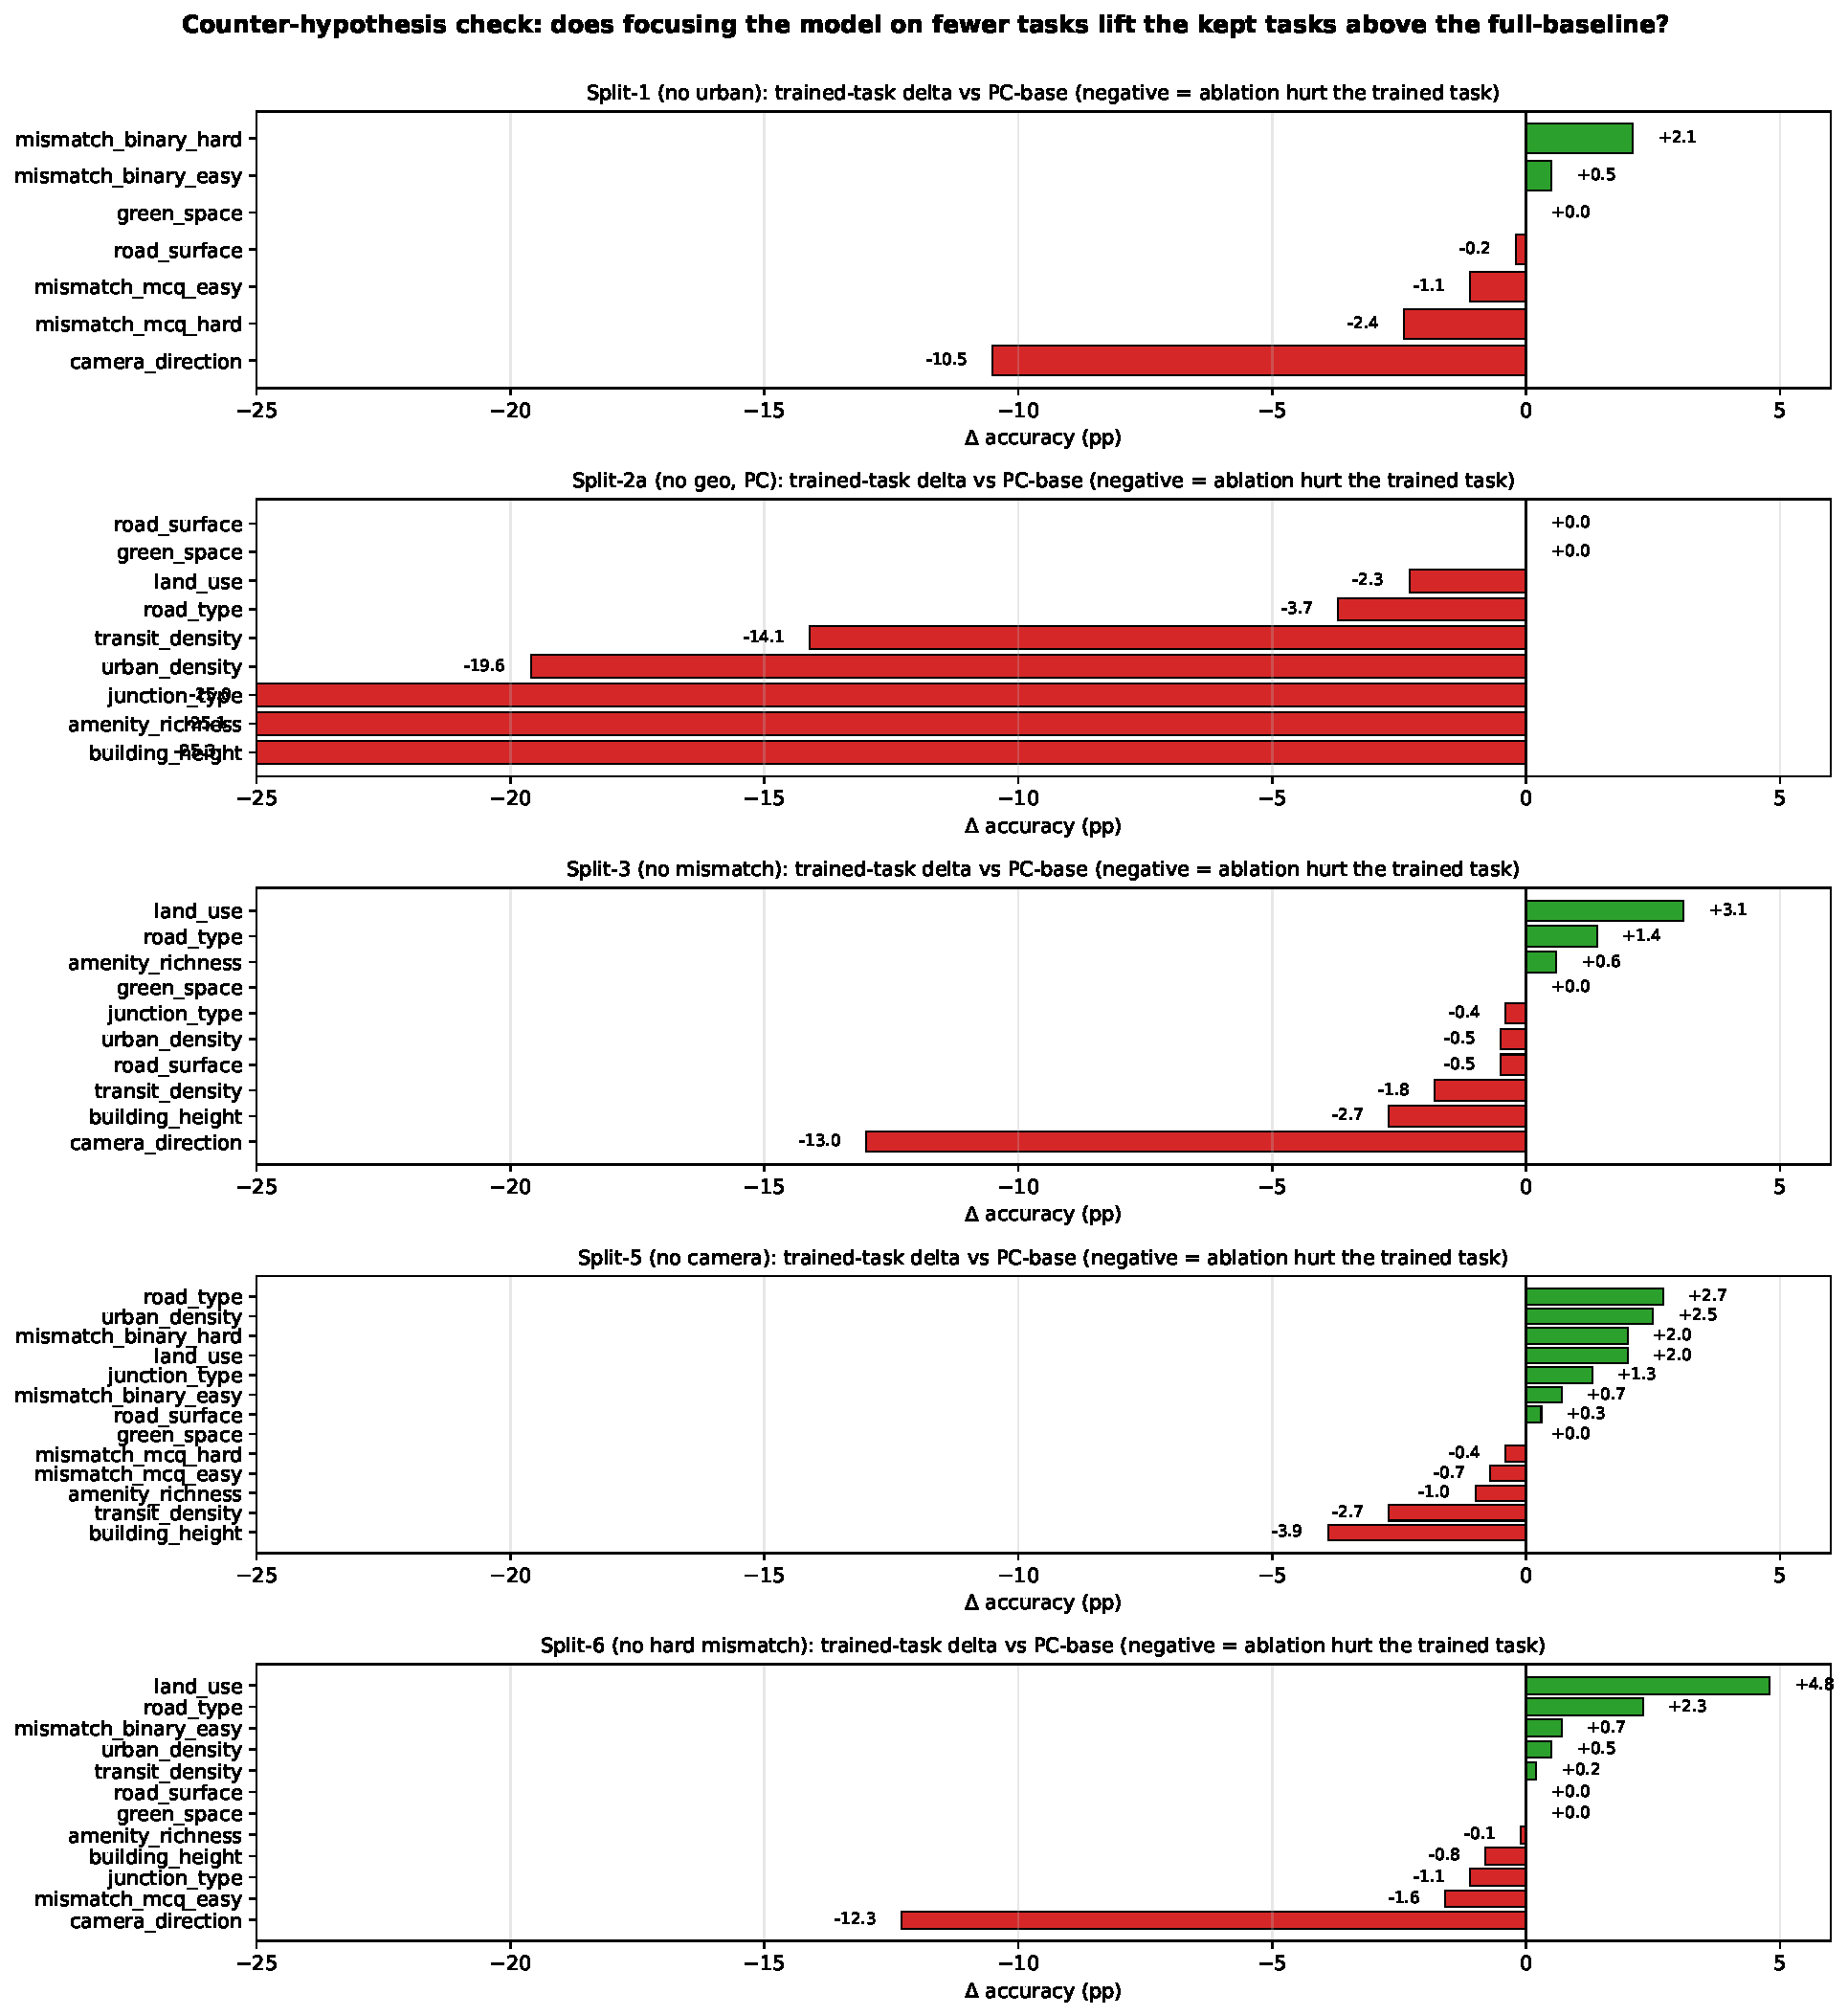
\includegraphics[width=0.95\textwidth]{figures/fig4_trained_vs_baseline.pdf}
\end{figure}

\begin{table}[h]\centering\small
\setlength{\tabcolsep}{6pt}
\begin{tabular}{l c r l}
\toprule
\textbf{Run} & \textbf{N kept} & \textbf{Mean $\Delta$ (pp)} & \textbf{Worst topic ($\Delta$)} \\
\midrule
Split-1                & 7  & \bad{$-1.6$}  & camera\_direction ($-10.5$) \\
Split-2a               & 9  & \bad{$-17.6$} & junction\_type ($-25.0$); urban\_density ($-19.6$) \\
Split-3                & 10 & \bad{$-3.6$}  & camera\_direction ($-13.0$); land\_use ($+3.1$) \\
Split-5                & 13 & \bad{$-1.8$}  & amenity\_richness ($-1.0$); urban\_density ($+2.5$) \\
Split-6                & 12 & \bad{$-2.0$}  & camera\_direction ($-12.3$); land\_use ($+4.8$) \\
\bottomrule
\end{tabular}
\end{table}

\begin{itemize}\itemsep1pt
\item Joint training beats focused training on every kept-task subset.
\item Smaller withholdings (Split-5,6) cost only $\sim$2 pp on kept tasks; large ones (Split-2a) cost $\sim$18 pp via training collapse.
\item Model is not capacity-limited per-task; cross-topic gradient mixing helps.
\end{itemize}

\newpage
\section{Withheld urban tasks (Split-1)}

\begin{figure}[h]\centering
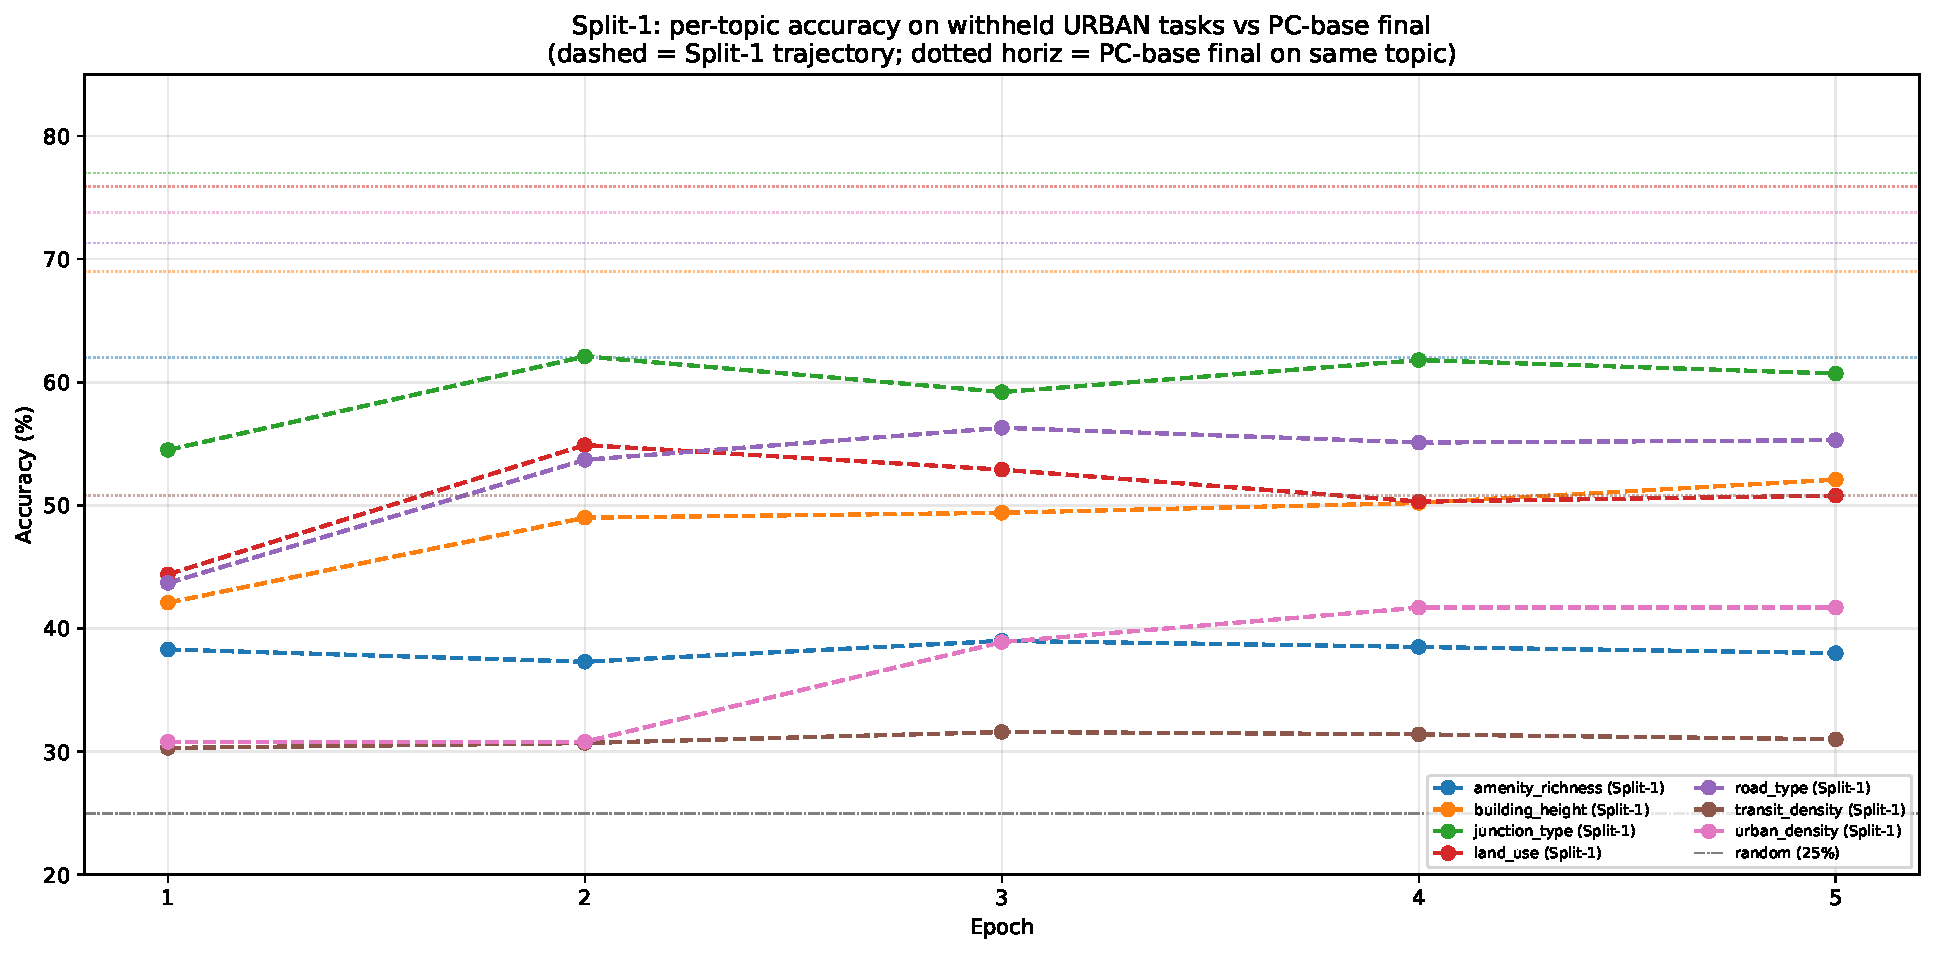
\includegraphics[width=\textwidth]{figures/fig2_split1_withheld.pdf}
\end{figure}

\begin{table}[h]\centering\small
\setlength{\tabcolsep}{6pt}
\begin{tabular}{l r r r r}
\toprule
\textbf{Topic} & \textbf{Split-1} & \textbf{PC-base} & \textbf{$\Delta$} & \textbf{vs random} \\
\midrule
amenity\_richness   & 38.0 & 62.0 & \bad{$-24.0$} & +13.0 \\
building\_height    & 52.1 & 69.0 & \bad{$-16.9$} & +27.1 \\
junction\_type      & 60.7 & 77.0 & \bad{$-16.3$} & +35.7 \\
land\_use           & 50.8 & 75.9 & \bad{$-25.1$} & +25.8 \\
road\_type          & 55.3 & 71.3 & \bad{$-16.0$} & +30.3 \\
transit\_density    & 31.0 & 50.8 & \bad{$-19.8$} & +6.0 \\
urban\_density      & 41.7 & 73.8 & \bad{$-32.1$} & +16.7 \\
\midrule
\textbf{Mean}       & \textbf{47.1} & \textbf{68.5} & \bad{$-21.4$} & +22.1 \\
\bottomrule
\end{tabular}
\end{table}

\begin{itemize}\itemsep1pt
\item Every urban topic lands between random and baseline; never above.
\item transit\_density: +6 over random --- weakest transfer.
\item urban\_density: $-32$ pp gap --- needs direct supervision.
\item Most urban topics plateau by ep3--4. More training does not close the gap.
\end{itemize}

\newpage
\section{Withheld mismatch + camera\_direction (Split-2a/2b/3/5/6)}

\begin{figure}[h]\centering
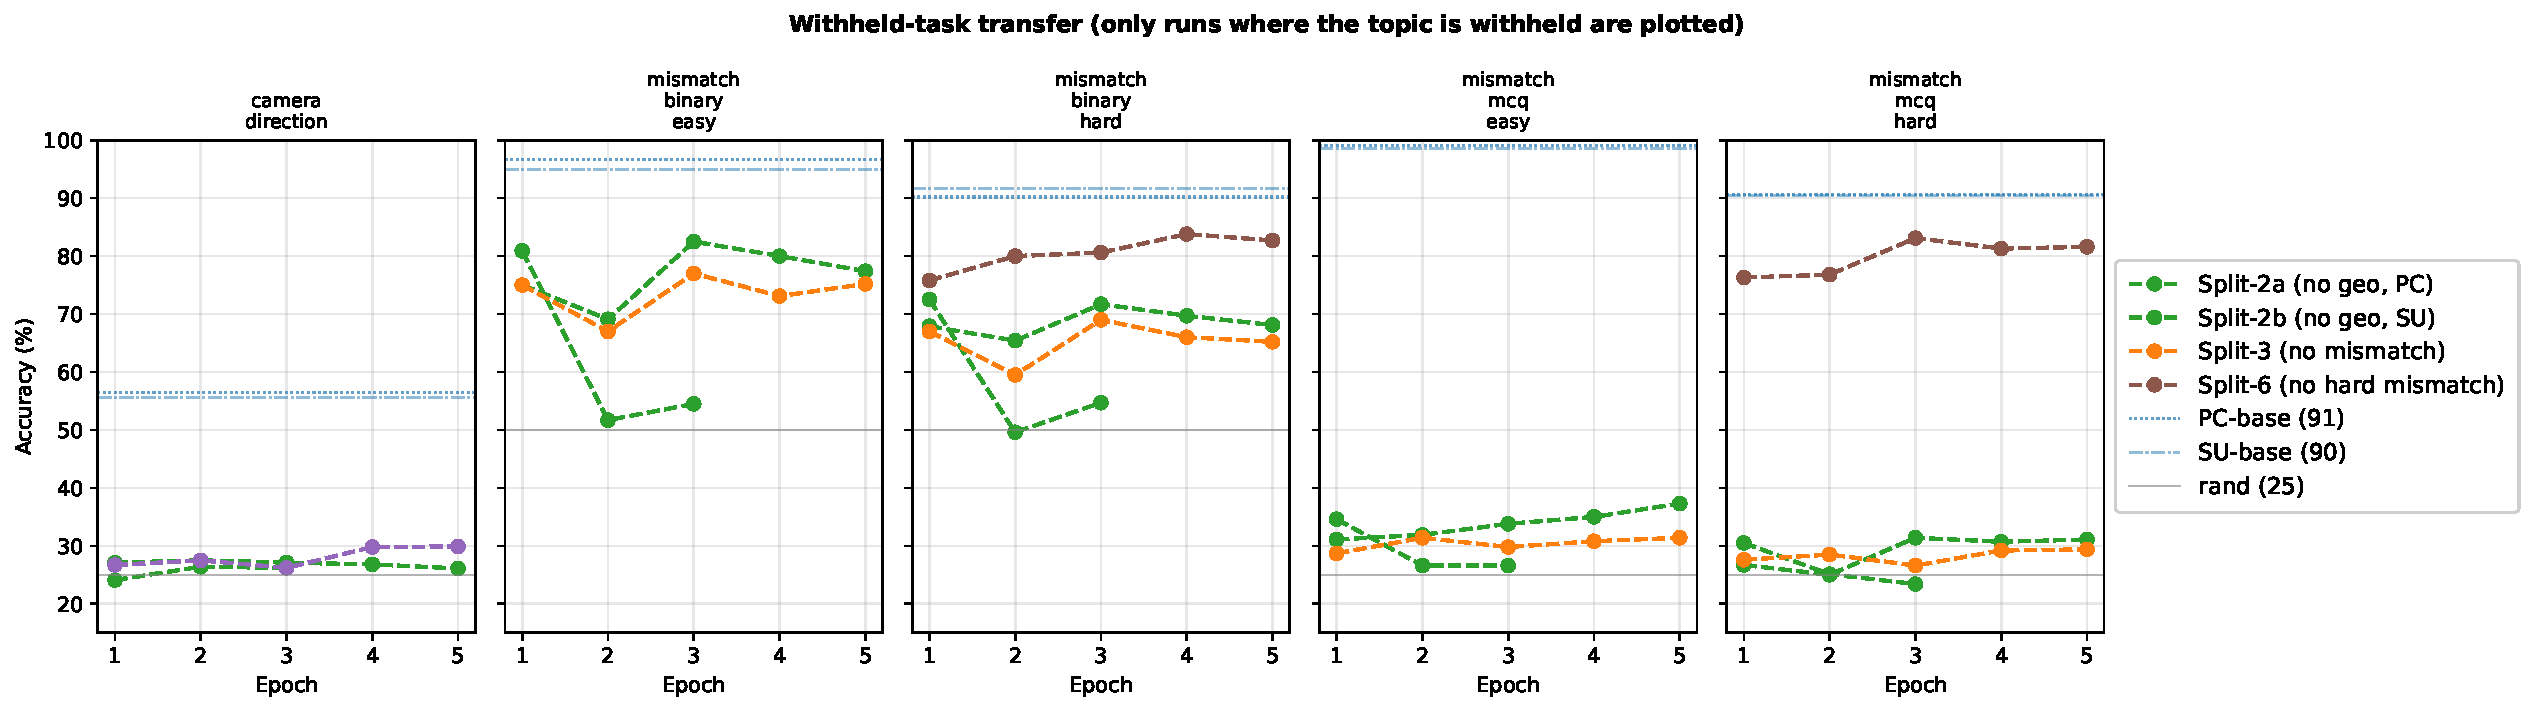
\includegraphics[width=\textwidth]{figures/fig3_geo_withheld.pdf}
\end{figure}

\begin{itemize}\itemsep1pt
\item mismatch\_mcq\_*: collapses to chance ($\sim$23--37\%, random=25) when the whole family is withheld (2a/2b/3). Unlearnable from urban supervision.
\item mismatch\_binary\_*: 65--77\% under family-withholding (random=50, baseline 90+). Partial transfer.
\item camera\_direction (full withhold, 2a/2b/5): stalls at 26--30\%, $\sim$random. Zero transfer from any other supervision in this dataset.
\item \textbf{Split-6: hard-only withholding nearly recovers}: mismatch\_binary\_hard 82.7\% (vs 54.7\% in 2a, 65.2\% in 3); mismatch\_mcq\_hard 81.6\% (vs 23.4\% in 2a, 29.4\% in 3). Easy variants of the same family carry the hard ones.
\item Split-2b recovers more than Split-2a on mismatch (77.4 vs 54.5 binary\_easy) --- larger train set + no early-stop collapse.
\item Split-3 final (ep5) confirms ep3 trend: mismatch\_mcq\_easy 31.4, hard 29.4 --- camera\_dir supervision does not help mismatch\_mcq.
\end{itemize}

\newpage
\section{Saturation}

\begin{table}[h]\centering\small
\setlength{\tabcolsep}{6pt}
\renewcommand{\arraystretch}{1.15}
\begin{tabular}{l l l l l}
\toprule
\textbf{Run} & \textbf{Last delta} & \textbf{Plateau ep} & \textbf{Trend} & \textbf{Auto verdict} \\
\midrule
PC-base    & ep5$\to$6: $+1.4$    & not reached       & \good{climbing}    & ``still improving'' \\
SU-base    & ep7$\to$8: $-1.4$    & ep4 (72.4)        & late drift         & ``plateauing'' \\
Split-1    & ep4$\to$5: $+0.2$    & ep4               & \good{plateaued}   & ``still improving'' (misleading) \\
Split-2a   & ep1 best (59.5)      & regressed         & \bad{collapsed}    & ``still improving'' (wrong) \\
Split-2b   & ep4$\to$5: $-0.5$    & ep3 (61.8)        & plateau            & ``plateauing'' \\
Split-3    & ep4$\to$5: $+0.6$    & ep3--5            & flat               & ``still improving'' (marginal) \\
Split-5    & ep4$\to$5: $+0.6$    & ep3--5            & flat               & ``still improving'' (marginal) \\
Split-6    & ep4$\to$5: $+0.1$    & ep3--5            & flat               & ``still improving'' (marginal) \\
\bottomrule
\end{tabular}
\end{table}

\begin{itemize}\itemsep1pt
\item Auto verdict only checks last-epoch delta. It misses Split-2a's collapse. Use the trajectory plots.
\end{itemize}

\section{Leakage flags}\label{sec:leakage}

\begin{figure}[h]\centering
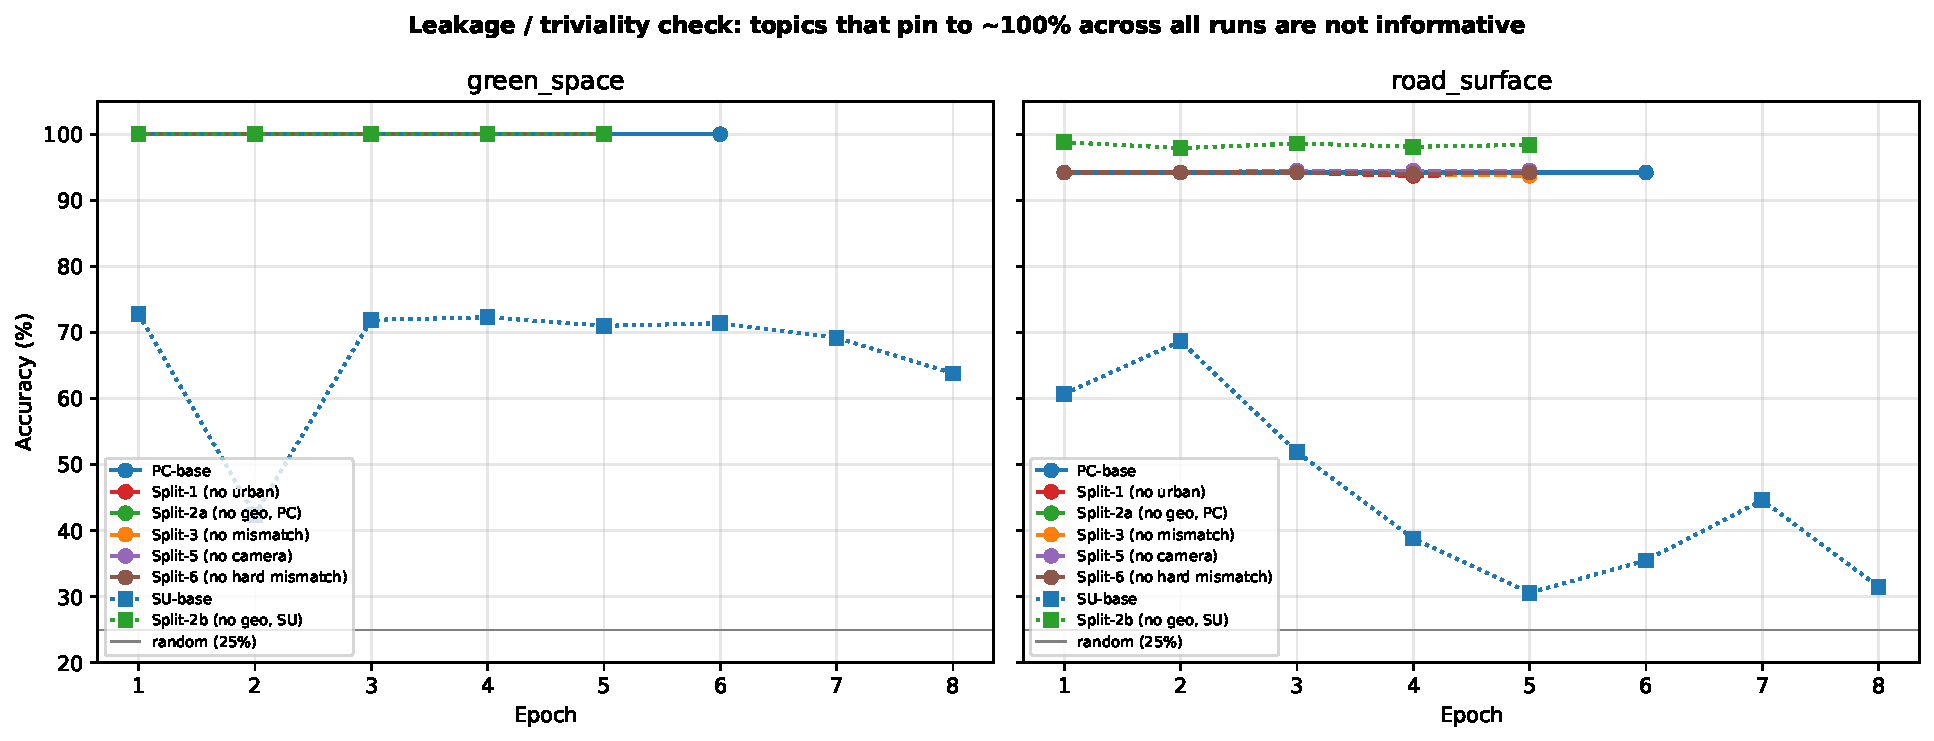
\includegraphics[width=\textwidth]{figures/fig5_leakage.pdf}
\end{figure}

\begin{itemize}\itemsep1pt
\item green\_space: 100\% in every per\_city run, including ablations. SU drops to 63.8 --- per\_city behavior is leakage.
\item road\_surface: pinned at 94.2 across consecutive epochs in PC --- non-vision prior. SU tanks to 31.5.
\item Either drop these from headline averages or report ``informative-topic average''.
\end{itemize}

\begin{table}[h]\centering\small
\setlength{\tabcolsep}{6pt}
\begin{tabular}{l c c c c c c c c}
\toprule
& PC-base & SU-base & Split-1 & Split-2a & Split-2b & Split-3 & Split-5 & Split-6 \\
\midrule
Mean over 12 non-trivial topics & 73.7 & 65.6 & 60.9 & 47.0 & 56.4 & 59.6 & 73.0 & 74.1 \\
\bottomrule
\end{tabular}
\end{table}

PC-base advantage over SU-base persists (+8.1 pp). Split-5/6 sit nearly even with PC-base on non-trivial topics --- single-topic withholdings have small overall cost.

\newpage
\section{Per-run verdicts: how trained tasks influenced unseen tasks}
\label{sec:per-run}

For each run, ``trained'' = topics with supervision in that run; ``withheld'' = topics held out and evaluated zero-shot. \textbf{$\Delta$ vs PC-base} is the gap on the same withheld topic between this run's zero-shot performance and PC-base's supervised performance --- it isolates the transfer cost of withholding. \textbf{$\Delta$ vs random} measures whether transfer beats chance.

\subsection*{PC-base (full, 14 topics, 6 ep) --- reference}

\begin{itemize}\itemsep1pt
\item No withholding. 78.3\% overall, still climbing at ep6.
\item Sets the ceiling every ablation is measured against. Mean of 12 informative topics: 73.7\%.
\item amenity\_richness, transit\_density are the hardest \emph{trained} topics (62, 51) --- training does not solve them. urban\_density jumps to 75.9 only by ep5 then drops.
\end{itemize}

\subsection*{SU-base (full, seen\_unseen, 8 ep) --- cross-city ceiling}

\begin{itemize}\itemsep1pt
\item All 14 trained, but evaluated on held-out cities. 70.8\% overall (best ep4: 72.4).
\item road\_surface and green\_space drop hard (94.2$\to$31.5; 100$\to$63.8): per\_city pinning is leakage; SU exposes it.
\item transit\_density falls 50.8$\to$36.9 cross-city; urban\_density holds at 70.6.
\item Verdict: SU-base is the honest headline. PC-vs-SU gap = +7.5 pp $\approx$ pure city-leakage premium.
\end{itemize}

\subsection*{Split-1 (withheld 7 urban) --- can geo supervision teach urban?}

Trained: 7 geo (camera\_dir, green\_space, road\_surface, 4 mismatch). Withheld: 7 urban.

\begin{itemize}\itemsep1pt
\item Overall 66.3 (vs PC-base 78.3). Trained tasks intact ($\geq$baseline on all 7 geo).
\item \textbf{Withheld urban: $-21.4$ pp on average} but \textbf{+22 pp over random}. Partial transfer, never recovery.
\item Best transfer: junction\_type (60.7, $-16.3$ pp), road\_type (55.3, $-16.0$). Both lean on visual scene understanding shared with road\_surface and mismatch.
\item Worst transfer: transit\_density (31.0, $\sim$random) --- requires explicit supervision; geo training gives \emph{nothing}.
\item urban\_density: 41.7 ($-32.1$ pp). The single biggest transfer failure.
\item amenity\_richness flat at 38\% all 5 ep (no learning curve at all on this withheld topic).
\item \textbf{Verdict: geo supervision $\to$ urban tasks is shallow. Transfer happens for spatial-layout topics, fails for count/density topics.}
\end{itemize}

\subsection*{Split-2a (withheld 5 geo, per\_city) --- can urban supervision teach geo?}

Trained: 9 urban + green\_space + road\_surface. Withheld: camera\_dir + 4 mismatch.

\begin{itemize}\itemsep1pt
\item Overall 50.7 (best ep1 = 59.5, then collapse). Worst-trained run.
\item Multiple \emph{trained} topics regressed 10--25 pp: junction\_type 67.9$\to$52, urban\_density 62$\to$54, mismatch\_binary\_easy 80.9$\to$54.5. mismatch\_binary\_easy was still in train set, so this is genuine training instability, not transfer.
\item Withheld camera\_dir: 26.2 (random=25). Zero transfer.
\item Withheld mismatch\_mcq\_*: 23--27\% (random=25). Zero transfer.
\item Withheld mismatch\_binary\_*: 54.5--54.7\% (random=50). $\sim$+5 pp over random --- minimal.
\item \textbf{Verdict: removing both mismatch and camera together destabilizes training; transfer to either is essentially nil. Do not interpret as ``urban knowledge does not help geo'' --- the run never converged.}
\end{itemize}

\subsection*{Split-2b (withheld 5 geo, seen\_unseen) --- same withholding, larger / more diverse train set}

\begin{itemize}\itemsep1pt
\item Overall 60.4 (best ep3 = 61.8). Stable, unlike 2a.
\item Withheld camera\_dir: 26.1 (random=25). Same zero transfer as 2a.
\item Withheld mismatch\_binary: 68--77\% (vs 2a 55\%, baseline 90+). Better than 2a because training did not collapse, but still $\sim$20 pp below baseline.
\item Withheld mismatch\_mcq: 31--37\% (random=25). Slow climb over epochs --- some weak transfer; still far from baseline 90\%.
\item \textbf{Verdict: with stable training, urban supervision lifts mismatch\_binary modestly and mismatch\_mcq slightly above chance. camera\_direction is unreachable from urban supervision regardless.}
\end{itemize}

\subsection*{Split-3 (withheld 4 mismatch, camera\_dir kept) --- isolates the mismatch family}

Trained: 9 urban + green\_space + road\_surface + camera\_direction. Withheld: 4 mismatch\_*.

\begin{itemize}\itemsep1pt
\item Overall 63.2 (5 ep). Trained tasks $\sim$$-3$ pp vs PC-base on average; camera\_dir lands at 43.5 vs PC-base 56.5 ($-13$ pp) --- camera\_dir benefits from mismatch supervision being present.
\item Withheld mismatch\_binary: 65.2--75.2\% (random=50). Partial transfer.
\item Withheld mismatch\_mcq: 29--31\% (random=25). \textbf{Stuck at chance for all 5 epochs} --- camera\_dir supervision does not unlock mismatch\_mcq.
\item Cross-check vs Split-2a: mismatch\_binary in Split-3 (65--75) > Split-2a (55) but $\approx$ Split-2b (68--77). Split-2b's improvement was training stability, not camera\_dir.
\item \textbf{Verdict: mismatch\_mcq is independently structured; no transfer source in this dataset reaches it. mismatch\_binary gets $\sim$15--25 pp from any non-collapsed training, regardless of which other tasks are present.}
\end{itemize}

\subsection*{Split-5 (withheld camera\_direction only) --- isolates camera\_dir transfer}

Trained: 13 (everything except camera\_direction). Withheld: camera\_direction.

\begin{itemize}\itemsep1pt
\item Overall 76.5 (vs PC-base 78.3). Smallest training-set delta of any ablation.
\item Trained tasks $\sim$$-1.8$ pp vs PC-base on average --- closest to baseline of any ablation.
\item Withheld camera\_direction: 26.7 $\to$ 29.9 over 5 epochs (random=25, baseline 56.5). \textbf{$\sim$random, $-26.6$ pp vs baseline.}
\item This is the cleanest measurement we have: with 13 supervised topics including all 4 mismatch + green\_space + road\_surface + 7 urban, camera\_direction still doesn't transfer at all.
\item \textbf{Verdict: camera\_direction has zero transfer source in this dataset. It must be supervised directly. The other 13 topics share no useful representation for it.}
\end{itemize}

\subsection*{Split-6 (withheld hard mismatch only) --- does the easy variant teach the hard one?}

Trained: 12 (drops mismatch\_binary\_hard + mismatch\_mcq\_hard). Withheld: 2 hard mismatch.

\begin{itemize}\itemsep1pt
\item Overall 76.4 (vs PC-base 78.3). Tied with Split-5 for smallest cost.
\item Withheld mismatch\_binary\_hard: \textbf{82.7\%} (random=50, baseline 90.2, $-7.5$ pp). Strong transfer.
\item Withheld mismatch\_mcq\_hard: \textbf{81.6\%} (random=25, baseline 90.6, $-9.0$ pp). Strong transfer.
\item Compare to Split-2a (whole family withheld): hard\_binary 54.7, hard\_mcq 23.4. Easy-variant supervision recovers $\sim$28--58 pp on the hard variant.
\item \textbf{Verdict: easy and hard mismatch share representation almost completely. Hard variants are not a separate learnable skill --- they are easy variants under harder distractors. This is the strongest positive transfer result in the study.}
\end{itemize}

\subsection*{Cross-cutting transfer summary}

\begin{table}[h]\centering\small
\setlength{\tabcolsep}{4pt}
\begin{tabular}{l l c c c}
\toprule
\textbf{Withheld topic} & \textbf{Run} & \textbf{Withheld acc} & \textbf{vs PC-base} & \textbf{vs random} \\
\midrule
camera\_direction       & Split-5 (only that)         & 29.9 & \bad{$-26.6$} & +4.9 \\
camera\_direction       & Split-2a (with mismatch)    & 26.2 & \bad{$-30.3$} & +1.2 \\
camera\_direction       & Split-2b (SU)               & 26.1 & \bad{$-29.5$} & +1.1 \\
\midrule
mismatch\_mcq\_easy     & Split-3 (whole family out)  & 31.4 & \bad{$-67.7$} & +6.4 \\
mismatch\_mcq\_easy     & Split-2a                    & 26.6 & \bad{$-72.5$} & +1.6 \\
mismatch\_mcq\_easy     & Split-2b (SU)               & 37.3 & \bad{$-61.2$} & +12.3 \\
\midrule
mismatch\_mcq\_hard     & Split-3                     & 29.4 & \bad{$-61.2$} & +4.4 \\
mismatch\_mcq\_hard     & Split-2a                    & 23.4 & \bad{$-67.2$} & $-1.6$ \\
mismatch\_mcq\_hard     & Split-2b (SU)               & 31.1 & \bad{$-59.4$} & +6.1 \\
mismatch\_mcq\_hard     & \textbf{Split-6 (only hard out)} & \good{81.6} & \good{$-9.0$} & +56.6 \\
\midrule
mismatch\_binary\_easy  & Split-3                     & 75.2 & \bad{$-21.4$} & +25.2 \\
mismatch\_binary\_easy  & Split-2a                    & 54.5 & \bad{$-42.1$} & +4.5 \\
mismatch\_binary\_easy  & Split-2b (SU)               & 77.4 & \bad{$-17.6$} & +27.4 \\
\midrule
mismatch\_binary\_hard  & Split-3                     & 65.2 & \bad{$-25.0$} & +15.2 \\
mismatch\_binary\_hard  & Split-2a                    & 54.7 & \bad{$-35.5$} & +4.7 \\
mismatch\_binary\_hard  & \textbf{Split-6 (only hard out)} & \good{82.7} & \good{$-7.5$} & +32.7 \\
\midrule
urban\_density          & Split-1                     & 41.7 & \bad{$-32.1$} & +16.7 \\
land\_use               & Split-1                     & 50.8 & \bad{$-25.1$} & +25.8 \\
amenity\_richness       & Split-1                     & 38.0 & \bad{$-24.0$} & +13.0 \\
junction\_type          & Split-1                     & 60.7 & \bad{$-16.3$} & +35.7 \\
road\_type              & Split-1                     & 55.3 & \bad{$-16.0$} & +30.3 \\
transit\_density        & Split-1                     & 31.0 & \bad{$-19.8$} & +6.0 \\
building\_height        & Split-1                     & 52.1 & \bad{$-16.9$} & +27.1 \\
\bottomrule
\end{tabular}
\end{table}

\begin{itemize}\itemsep1pt
\item \textbf{Three transfer regimes are visible}:
\begin{itemize}\itemsep0pt
\item \emph{Strong (within-family)}: easy$\to$hard mismatch (Split-6): $-7$ to $-9$ pp gap, $+30$ to $+57$ over random.
\item \emph{Partial (cross-family, structured)}: urban tasks under geo supervision (Split-1, Split-2b): $-16$ to $-25$ pp, $+10$ to $+35$ over random.
\item \emph{None}: camera\_direction under any supervision; mismatch\_mcq when whole family withheld --- both essentially at random.
\end{itemize}
\item Topics with \emph{strong cross-family} transfer in this dataset: junction\_type, road\_type (mostly visual scene cues).
\item Topics with \emph{no transfer source}: camera\_direction, transit\_density, mismatch\_mcq.
\item Practical implication: when curating a smaller training mix, the \emph{family} matters more than the count. Dropping one topic from a family is cheap; dropping the whole family is catastrophic.
\end{itemize}

\newpage
\section{For the paper}

\textbf{Report:}
\begin{itemize}\itemsep1pt
\item Joint training beats focused training on every kept-task subset.
\item Three transfer regimes: strong within-family (easy$\to$hard mismatch, $-8$ pp), partial cross-family for spatial-layout tasks ($-16$ to $-25$ pp), none for camera\_direction or mismatch\_mcq when family withheld ($\sim$random).
\item mismatch\_mcq + camera\_direction need direct supervision; they are not transfer targets.
\item Urban tasks transfer partially: +22 pp over random when withheld, but $\sim$20 pp below baseline.
\item Cross-city eval costs $\sim$7--8 pp uniformly. Use SU-base (70.8\%) as the honest headline.
\item green\_space, road\_surface are leaked on per\_city. Flag or exclude.
\end{itemize}

\textbf{Do NOT claim:}
\begin{itemize}\itemsep1pt
\item ``Urban knowledge transfers to mismatch tasks'' --- mismatch\_mcq stays at chance whenever the whole family is withheld.
\item ``camera\_direction transfers'' --- Split-5 isolates this and shows $\sim$random with all 13 other topics supervised.
\item ``Ablation X is close to baseline'' --- different denominator topic sets.
\item Cite the auto verdict banner --- it is wrong for Split-2a.
\end{itemize}

\textbf{Suggested compact paper table:}

\begin{table}[h]\centering\small
\setlength{\tabcolsep}{4pt}
\begin{tabular}{l c c c c c}
\toprule
\textbf{Train mix} & \textbf{Eval} & \textbf{Overall} & \textbf{Trained mean} & \textbf{Withheld mean} & \textbf{vs random} \\
\midrule
all 14 (PC-base)                  & per\_city    & 78.3 & 78.3 & ---  & --- \\
all 14 (SU-base)                  & seen\_unseen & 70.8 & 70.8 & ---  & --- \\
geo only (Split-1)                & per\_city    & 66.3 & 91.4 & 47.1 & +22 \\
urban only PC (Split-2a)          & per\_city    & 50.7 & 65.4 & 37.0 & $\sim$+0 \\
urban only SU (Split-2b)          & seen\_unseen & 60.4 & 70.4 & 48.0 & $\sim$+10 \\
urban+cam (Split-3)               & per\_city    & 63.2 & 76.0 & 50.4 & +8 \\
no camera (Split-5)               & per\_city    & 76.5 & 80.1 & 29.9 & +5 \\
no hard mismatch (Split-6)        & per\_city    & 76.4 & 79.6 & 82.2 & +32 \\
\bottomrule
\end{tabular}
\end{table}

mismatch\_binary random=50; mismatch\_mcq, camera=25. Withheld mean uses only the topics dropped from that run.

\appendix
\newpage
\section{Per-epoch trajectories}\label{app:per-epoch}

\subsection*{PC-base (per\_city, 6 ep)}

\begin{table}[h]\centering\scriptsize
\setlength{\tabcolsep}{5pt}
\begin{tabular}{l c c c c c c}
\toprule
& ep1 & ep2 & ep3 & ep4 & ep5 & ep6 \\
\midrule
\textbf{Overall}      & 71.5 & 72.3 & 75.0 & 76.4 & 76.9 & \textbf{78.3} \\
amenity\_richness     & 49.2 & 49.2 & 51.9 & 57.2 & 53.5 & 62.0 \\
building\_height      & 62.5 & 60.2 & 60.2 & 65.1 & 64.4 & 69.0 \\
camera\_direction     & 25.3 & 35.1 & 46.0 & 51.0 & 53.1 & 56.5 \\
green\_space          & 100.0 & 100.0 & 100.0 & 100.0 & 100.0 & 100.0 \\
junction\_type        & 69.9 & 71.7 & 72.8 & 76.6 & 70.1 & 77.0 \\
land\_use             & 76.8 & 75.9 & 76.5 & 77.0 & 77.5 & 75.9 \\
mismatch\_binary\_easy& 91.6 & 93.6 & 96.3 & 94.5 & 96.8 & 96.6 \\
mismatch\_binary\_hard& 87.2 & 85.0 & 88.6 & 88.8 & 92.0 & 90.2 \\
mismatch\_mcq\_easy   & 95.0 & 94.3 & 96.8 & 98.2 & 98.0 & 99.1 \\
mismatch\_mcq\_hard   & 82.7 & 81.5 & 86.8 & 88.2 & 90.6 & 90.6 \\
road\_surface         & 94.2 & 94.2 & 94.2 & 94.2 & 94.2 & 94.2 \\
road\_type            & 73.3 & 71.1 & 73.1 & 74.7 & 71.3 & 71.3 \\
transit\_density      & 44.6 & 44.9 & 44.6 & 47.2 & 48.5 & 50.8 \\
urban\_density        & 65.1 & 69.5 & 72.5 & 68.3 & 75.9 & 73.8 \\
\bottomrule
\end{tabular}
\end{table}

\subsection*{SU-base (seen\_unseen, 8 ep, early-stopped)}

\begin{table}[h]\centering\scriptsize
\setlength{\tabcolsep}{4pt}
\begin{tabular}{l c c c c c c c c}
\toprule
& ep1 & ep2 & ep3 & ep4 & ep5 & ep6 & ep7 & ep8 \\
\midrule
\textbf{Overall}      & 67.2 & 66.0 & 70.7 & \textbf{72.4} & 71.9 & 72.5 & 72.2 & 70.8 \\
amenity\_richness     & 57.8 & 35.7 & 61.6 & 65.4 & 54.5 & 63.6 & 61.6 & 59.4 \\
building\_height      & 44.1 & 43.8 & 51.8 & 55.9 & 54.0 & 54.8 & 52.6 & 54.4 \\
camera\_direction     & 26.5 & 28.7 & 42.5 & 48.0 & 55.5 & 57.0 & 56.7 & 55.6 \\
green\_space          & 72.8 & 42.4 & 71.9 & 72.3 & 71.0 & 71.4 & 69.2 & 63.8 \\
junction\_type        & 72.7 & 68.3 & 67.5 & 68.1 & 75.6 & 69.4 & 69.2 & 71.4 \\
land\_use             & 70.8 & 72.9 & 69.1 & 74.2 & 74.7 & 71.4 & 71.0 & 69.1 \\
mismatch\_binary\_easy& 93.5 & 93.5 & 94.0 & 93.8 & 96.2 & 95.9 & 97.3 & 95.0 \\
mismatch\_binary\_hard& 81.5 & 81.2 & 86.3 & 89.7 & 89.0 & 91.1 & 92.6 & 91.6 \\
mismatch\_mcq\_easy   & 89.6 & 95.8 & 95.3 & 97.6 & 98.1 & 98.0 & 98.1 & 98.5 \\
mismatch\_mcq\_hard   & 78.9 & 82.9 & 81.9 & 87.4 & 87.7 & 88.9 & 91.1 & 90.5 \\
road\_surface         & 60.7 & 68.7 & 51.9 & 38.8 & 30.6 & 35.5 & 44.6 & 31.5 \\
road\_type            & 71.4 & 72.3 & 70.0 & 70.8 & 73.1 & 70.4 & 67.7 & 70.9 \\
transit\_density      & 46.5 & 38.7 & 49.5 & 50.6 & 47.2 & 46.5 & 41.3 & 36.9 \\
urban\_density        & 62.5 & 70.1 & 76.5 & 75.6 & 70.9 & 72.4 & 70.4 & 70.6 \\
\bottomrule
\end{tabular}
\end{table}

road\_surface degrades 60.7$\to$31.5 over 8 epochs --- model overfits per-city prior, breaks cross-city.

\newpage
\subsection*{Split-1 (no urban, 5 ep)}

\begin{table}[h]\centering\scriptsize
\setlength{\tabcolsep}{6pt}
\begin{tabular}{l c c c c c}
\toprule
& ep1 & ep2 & ep3 & ep4 & ep5 \\
\midrule
\textbf{Overall}      & 59.6 & 63.4 & 64.8 & 66.1 & \textbf{66.3} \\
amenity\_richness     & 38.3 & 37.3 & 39.0 & 38.5 & 38.0 \\
building\_height      & 42.1 & 49.0 & 49.4 & 50.2 & 52.1 \\
camera\_direction     & 26.0 & 31.4 & 40.5 & 41.9 & 46.0 \\
green\_space          & 100.0 & 100.0 & 100.0 & 100.0 & 100.0 \\
junction\_type        & 54.5 & 62.1 & 59.2 & 61.8 & 60.7 \\
land\_use             & 44.4 & 54.9 & 52.9 & 50.3 & 50.8 \\
mismatch\_binary\_easy& 94.5 & 96.4 & 92.7 & 98.0 & 97.1 \\
mismatch\_binary\_hard& 84.0 & 89.1 & 87.5 & 92.7 & 92.3 \\
mismatch\_mcq\_easy   & 93.6 & 95.2 & 97.1 & 97.9 & 98.0 \\
mismatch\_mcq\_hard   & 79.3 & 83.1 & 86.1 & 88.4 & 88.2 \\
road\_surface         & 94.2 & 94.2 & 94.2 & 93.7 & 94.0 \\
road\_type            & 43.7 & 53.7 & 56.3 & 55.1 & 55.3 \\
transit\_density      & 30.3 & 30.7 & 31.6 & 31.4 & 31.0 \\
urban\_density        & 30.8 & 30.8 & 38.9 & 41.7 & 41.7 \\
\bottomrule
\end{tabular}
\end{table}

transit\_density flat 30--31\% all 5 epochs; amenity\_richness flat $\sim$38\%. Geo-only training has zero signal here.

\subsection*{Split-2a (no geo, PC --- regressed)}

\begin{table}[h]\centering\scriptsize
\setlength{\tabcolsep}{8pt}
\begin{tabular}{l c c c}
\toprule
& ep1 & ep2 & ep3 \\
\midrule
\textbf{Overall}      & \textbf{59.5} & 50.4 & 50.7 \\
amenity\_richness     & 50.4 & 36.2 & 36.9 \\
building\_height      & 60.5 & 44.4 & 43.7 \\
camera\_direction     & 24.1 & 26.4 & 26.2 \\
green\_space          & 100.0 & 100.0 & 100.0 \\
junction\_type        & 67.9 & 58.3 & 52.0 \\
land\_use             & 76.3 & 72.9 & 73.6 \\
mismatch\_binary\_easy& 80.9 & 51.7 & 54.5 \\
mismatch\_binary\_hard& 72.5 & 49.6 & 54.7 \\
mismatch\_mcq\_easy   & 34.6 & 26.6 & 26.6 \\
mismatch\_mcq\_hard   & 30.5 & 25.1 & 23.4 \\
road\_surface         & 94.2 & 94.2 & 94.2 \\
road\_type            & 72.0 & 66.8 & 67.6 \\
transit\_density      & 39.9 & 34.9 & 36.7 \\
urban\_density        & 62.2 & 55.1 & 54.2 \\
\bottomrule
\end{tabular}
\end{table}

ep1 was best; multiple trained tasks regressed 10+ pp afterward.

\newpage
\subsection*{Split-2b (no geo, SU)}

\begin{table}[h]\centering\scriptsize
\setlength{\tabcolsep}{6pt}
\begin{tabular}{l c c c c c}
\toprule
& ep1 & ep2 & ep3 & ep4 & ep5 \\
\midrule
\textbf{Overall}      & 58.9 & 59.0 & \textbf{61.8} & 60.9 & 60.4 \\
amenity\_richness     & 58.1 & 61.7 & 62.9 & 60.4 & 59.7 \\
building\_height      & 47.1 & 50.4 & 51.1 & 53.7 & 54.0 \\
camera\_direction     & 27.1 & 27.5 & 27.1 & 26.8 & 26.1 \\
green\_space          & 100.0 & 100.0 & 100.0 & 100.0 & 100.0 \\
junction\_type        & 75.2 & 74.7 & 72.9 & 69.4 & 69.6 \\
land\_use             & 70.4 & 74.6 & 74.0 & 75.6 & 76.2 \\
mismatch\_binary\_easy& 75.0 & 69.1 & 82.5 & 80.0 & 77.4 \\
mismatch\_binary\_hard& 67.9 & 65.4 & 71.7 & 69.7 & 68.1 \\
mismatch\_mcq\_easy   & 31.1 & 31.9 & 33.8 & 35.0 & 37.3 \\
mismatch\_mcq\_hard   & 26.7 & 25.0 & 31.4 & 30.7 & 31.1 \\
road\_surface         & 98.8 & 97.9 & 98.6 & 98.1 & 98.4 \\
road\_type            & 73.1 & 71.7 & 72.7 & 71.3 & 72.1 \\
transit\_density      & 45.7 & 44.9 & 49.1 & 48.8 & 44.9 \\
urban\_density        & 71.3 & 75.0 & 75.8 & 73.3 & 72.9 \\
\bottomrule
\end{tabular}
\end{table}

Best ep3 (61.8); mild $-1.4$ drift. mismatch\_mcq slowly climbs ep1 31.1 $\to$ ep5 37.3 on transfer alone.

\subsection*{Split-3 (no mismatch, 5 ep)}

\begin{table}[h]\centering\scriptsize
\setlength{\tabcolsep}{6pt}
\begin{tabular}{l c c c c c}
\toprule
& ep1 & ep2 & ep3 & ep4 & ep5 \\
\midrule
\textbf{Overall}      & 57.8 & 59.3 & 62.7 & 62.6 & \textbf{63.2} \\
amenity\_richness     & 52.6 & 53.7 & 61.3 & 62.2 & 62.6 \\
building\_height      & 49.8 & 62.8 & 64.8 & 66.3 & 66.3 \\
camera\_direction     & 23.0 & 33.0 & 42.8 & 39.9 & 43.5 \\
green\_space          & 100.0 & 100.0 & 100.0 & 100.0 & 100.0 \\
junction\_type        & 66.1 & 71.4 & 74.6 & 75.4 & 76.6 \\
land\_use             & 76.1 & 76.5 & 77.9 & 80.7 & 79.0 \\
mismatch\_binary\_easy& 75.0 & 67.0 & 77.0 & 73.1 & 75.2 \\
mismatch\_binary\_hard& 67.0 & 59.5 & 69.0 & 66.0 & 65.2 \\
mismatch\_mcq\_easy   & 28.7 & 31.4 & 29.8 & 30.8 & 31.4 \\
mismatch\_mcq\_hard   & 27.6 & 28.5 & 26.6 & 29.2 & 29.4 \\
road\_surface         & 94.2 & 94.2 & 94.2 & 94.0 & 93.7 \\
road\_type            & 70.9 & 73.6 & 72.7 & 72.7 & 72.7 \\
transit\_density      & 45.6 & 44.6 & 47.4 & 46.2 & 49.0 \\
urban\_density        & 63.1 & 69.3 & 72.5 & 72.9 & 73.3 \\
\bottomrule
\end{tabular}
\end{table}

mismatch\_mcq stays near chance ($\sim$29\%) for all 5 epochs even with camera\_direction supervised. mismatch\_binary stuck at $\sim$65--75\%.

\subsection*{Split-5 (no camera\_direction, 5 ep)}

\begin{table}[h]\centering\scriptsize
\setlength{\tabcolsep}{6pt}
\begin{tabular}{l c c c c c}
\toprule
& ep1 & ep2 & ep3 & ep4 & ep5 \\
\midrule
\textbf{Overall}      & 70.7 & 71.8 & 74.9 & 75.9 & \textbf{76.5} \\
amenity\_richness     & 51.7 & 50.6 & 55.6 & 59.0 & 61.0 \\
building\_height      & 54.4 & 61.3 & 61.7 & 65.5 & 65.1 \\
camera\_direction     & 26.7 & 27.5 & 26.2 & 29.8 & 29.9 \\
green\_space          & 100.0 & 100.0 & 100.0 & 100.0 & 100.0 \\
junction\_type        & 69.0 & 72.3 & 75.9 & 77.0 & 78.3 \\
land\_use             & 75.6 & 75.6 & 78.6 & 77.5 & 77.9 \\
mismatch\_binary\_easy& 92.0 & 96.1 & 96.1 & 97.1 & 97.3 \\
mismatch\_binary\_hard& 86.5 & 83.6 & 90.0 & 91.4 & 92.2 \\
mismatch\_mcq\_easy   & 95.7 & 94.3 & 98.4 & 98.2 & 98.4 \\
mismatch\_mcq\_hard   & 81.6 & 82.7 & 88.4 & 90.6 & 90.2 \\
road\_surface         & 94.2 & 94.2 & 94.5 & 94.5 & 94.5 \\
road\_type            & 70.4 & 70.6 & 73.6 & 73.4 & 74.0 \\
transit\_density      & 44.6 & 45.5 & 48.3 & 48.0 & 48.1 \\
urban\_density        & 61.1 & 66.5 & 72.9 & 73.8 & 76.3 \\
\bottomrule
\end{tabular}
\end{table}

camera\_direction trajectory: 26.7$\to$29.9 over 5 epochs (random=25, baseline 56.5). Overall climbs +5.8 pp on the other 13 topics --- camera\_dir is not pulled along by capacity gains.

\newpage
\subsection*{Split-6 (no hard mismatch, 5 ep)}

\begin{table}[h]\centering\scriptsize
\setlength{\tabcolsep}{6pt}
\begin{tabular}{l c c c c c}
\toprule
& ep1 & ep2 & ep3 & ep4 & ep5 \\
\midrule
\textbf{Overall}      & 68.5 & 73.3 & 75.1 & 76.3 & \textbf{76.4} \\
amenity\_richness     & 47.8 & 58.6 & 58.3 & 59.9 & 61.9 \\
building\_height      & 61.3 & 57.9 & 62.5 & 65.9 & 68.2 \\
camera\_direction     & 25.8 & 41.7 & 39.9 & 45.1 & 44.2 \\
green\_space          & 100.0 & 100.0 & 100.0 & 100.0 & 100.0 \\
junction\_type        & 65.8 & 72.1 & 74.6 & 76.3 & 75.9 \\
land\_use             & 77.4 & 76.3 & 79.9 & 79.0 & 80.7 \\
mismatch\_binary\_easy& 93.2 & 95.7 & 96.8 & 97.3 & 97.3 \\
mismatch\_binary\_hard& 75.8 & 80.0 & 80.6 & 83.8 & 82.7 \\
mismatch\_mcq\_easy   & 93.0 & 95.5 & 97.0 & 98.0 & 97.5 \\
mismatch\_mcq\_hard   & 76.3 & 76.8 & 83.1 & 81.3 & 81.6 \\
road\_surface         & 94.2 & 94.2 & 94.2 & 94.0 & 94.2 \\
road\_type            & 66.7 & 70.1 & 73.3 & 73.6 & 73.6 \\
transit\_density      & 39.8 & 47.6 & 50.4 & 51.7 & 51.0 \\
urban\_density        & 61.0 & 71.7 & 72.2 & 74.0 & 74.3 \\
\bottomrule
\end{tabular}
\end{table}

Withheld hard variants reach 81--83\% by ep5 (vs $\sim$90\% in PC-base) --- only $\sim$8 pp gap. The easy variant of the same family carries the hard one almost fully.

\section{Method}

\begin{itemize}\itemsep1pt
\item Ablation runs: bs=96, NUM\_EPOCHS=5, early-stop patience=2, cosine LR, 100 warmup, LoRA r=16/$\alpha$=16, all-linear, SEED=3407, RTX Pro 6000 96 GB.
\item PC-base bs=86, 6 ep; SU-base bs=80, 8 ep --- earlier runs, same pipeline, identical eval routine.
\item Eval: greedy decoding, deterministic. PC=6984 samples, SU=8831.
\item Baselines per topic from verdict files: mismatch\_binary 2-way (rand=50), all others 4-way (rand=25).
\end{itemize}

\end{document}
